\documentclass[11pt,letterpaper]{article}
\usepackage{fullpage}
\usepackage{multicol}
\usepackage{amsmath}
\usepackage{amsfonts}
\usepackage{amssymb}
%\usepackage{pstricks, pst-node, pst-plot}

\ifx\pdfoutput\undefined
% we are running LaTeX, not pdflatex
\usepackage{graphicx}
\else
% we are running pdflatex, so convert .eps files to .pdf
\usepackage[pdftex]{graphicx}
\usepackage{epstopdf}
\fi

\newcommand{\ds}{\displaystyle}
\newcommand{\bv}{\mathbf}
\newcommand{\lv}{\langle}
\newcommand{\rv}{\rangle}

\begin{document}
\flushleft
\begin{multicols}{2}


\begin{large}\textbf{Math 116 Quiz 3: $\oint$ 7.5, 8.1-8.2 (sans arc length) \\
Tue 25 Sep 2012}\end{large}

\textbf{Name:  }\underline{\hspace{35ex}}

\vspace{.5in}

\end{multicols}

\pagestyle{empty}


\flushleft

You have 25 minutes to complete this quiz.  Eyes on your own paper and good luck!

\begin{enumerate}

\item \textbf{Definitions/Concepts.} (2 pts) Fill in the following inequalities using the symbols TRAP$(n)$ or MID$(n)$.  

\smallskip
If the graph of $f$ is concave down on $[a,b]$, then
\[\leq\int_a^bf(x)dx\leq\]
If the graph of $f$ is concave up on $[a,b]$, then
\[\leq\int_a^bf(x)dx\leq\]

\vspace{1pc}
\item \textbf{Questions/Problems.} (8 pts)
\noindent Let $S$ be the solid whose base is the region bounded by the graph of the curve $y=\frac{1}{\sqrt{x(1+a\ln\,x)}}$ (for some positive constant $a>0$), the $x$-axis, the lines $x=1$ and $x=e$.  The cross-sections of $S$ perpendicular to the $x$-axis are squares.  Find the exact volume of $S$.
\smallskip
\begin{center}
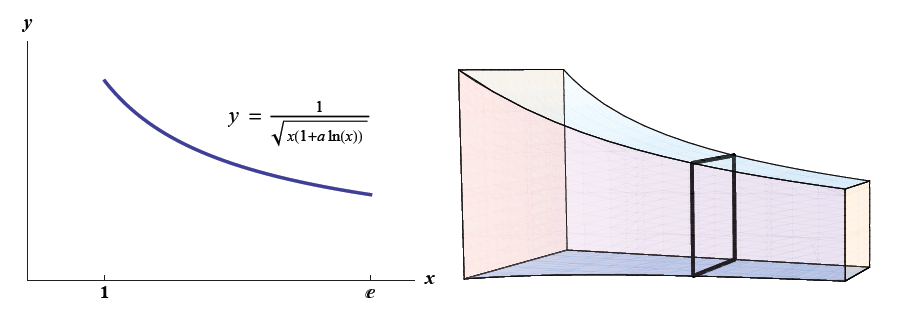
\includegraphics[width=.9\textwidth]{quiz3pic.png}
\end{center}
\vspace{10pc}
\vfill
\hfill{\bf MORE QUIZ ON THE BACK --\textgreater}

\item \textbf{Computations/Algebra.} 

\smallskip
\begin{enumerate} 
\item $\int_0^6\pi(3-y/2)^2dy$
\smallskip
\begin{enumerate}
\item (1 pt) Which shape is being integrated?  Choose one:
\begin{enumerate}
\item triangle
\item part of a circle
\item hemisphere
\item cone
\end{enumerate}
\smallskip
\item (2 pts) If you chose triangle, write down the base and height, indicating which is which.  If you chose part of a circle or hemisphere, write down the radius.  If you chose cone, write down the radius and the height, indicating which is which.

\vspace{3pc}
\item (2 pts) Draw a picture to justify your answers to parts i. and ii.

\vspace{6pc}
\end{enumerate}

\item $\int_{-9}^9\sqrt{81-x^2}dx$
\smallskip
\begin{enumerate}
\item (1 pt) Which shape is being integrated?  Choose one:
\begin{enumerate}
\item triangle
\item part of a circle
\item hemisphere
\item cone
\end{enumerate}
\smallskip
\item (2 pts) If you chose triangle, write down the base and height, indicating which is which.  If you chose part of a circle or hemisphere, write down the radius.  If you chose cone, write down the radius and the height, indicating which is which.

\vspace{3pc}
\item (2 pts) Draw a picture to justify your answers to parts i. and ii.

\vspace{6pc}
\end{enumerate}

\end{enumerate}

\end{enumerate}

{\bf ChAlLeNgE pRoBlEm:} Rotate the bell curve $y=e^{-x^2/2}$ around the $y$-axis, forming a hill-shaped solid of revolution.  Using horizontal slices, find the exact volume of this hill.

\end{document}


